%%%%%%%%%%% Aquí va la solución al problema 3.
\textbf{\textcolor{MidnightBlue}{3.}} Considera el algoritmo de consenso con
fallas de tipo paro visto en clase. Suponga que en lugar de ejecutar $f + 1$
rondas, el algoritmo sólo ejecuta $f$, con la misma regla de decisión. Describa
una ejecución particular en la que las propiedades de validez y acuerdo sean violadas.
\newline

\begin{center}
    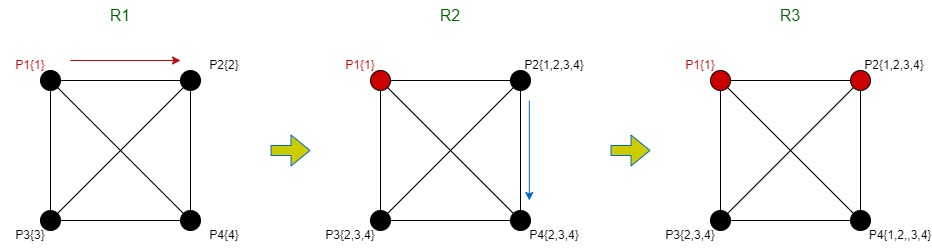
\includegraphics[scale=0.5]{Consenso.jpeg}
    \end{center}

$\rhd$ Para esta ejecución basta observar que puede pasar en cada
ronda si resultan $2$ fallos de tipo paro en un sistema distribuido
con $4$ procesos. Esto es
\begin{itemize}
\item $\mathbf{R_1}.$ Para esta ronda todos los procesos mandan su \code{ID}
      exceptuando al proceso $p_1$ que logra mandar su \code{ID} al proceso
      $p_2$ y después tiene un problema tipo fallo y no completa su envio a
      los demás procesos.
\item $\mathbf{R_2.}$ En la $2^{\text{da}}$ ronda el proceso $p_2$ manda su
      \code{ID} a $p_4$ pero no logra enviarselo al proceso $p_3$. Entonces
      $p_2$ es nuestro segundo proceso con fallo de tipo paro.
\end{itemize}
El algoritmo solo nos permite realizar $2$ rondas, pues $f = 2$. Así,
la vista de $p_3$ es $\{2, 3, 4\}$ y su propuesta es $prop = 2$. Mientras
que $p_4$ contiene en su vista a $\{1, 2, 3, 4\}$ y su propuesta es
$prop = 1$. Como se puede observar, los procesos restantes en el sistema
no han llegado a un consenso en $f$ rondas.
\hfill $\lhd$
